\documentclass[varwidth=true, border=2pt]{standalone}
\usepackage{tkz-euclide}
\usepackage{tikz}
\usetikzlibrary{shapes, calc, shapes, arrows}
\usepackage{amsmath,amssymb}

\usepackage{xcolor}
\definecolor{xvectorcolor}{HTML}{77933C}

\begin{document}
\usetkzobj{all}
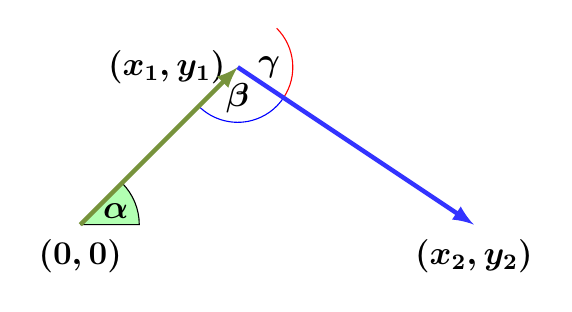
\begin{tikzpicture}[font=\boldmath]
    \large

    % Points
    \coordinate (A) at (0,0) {};
    \coordinate (B) at (2,2) {};
    \coordinate (AB2) at (3,3) {};
    \coordinate (C) at (5,0) {};

    \node[below of=A,node distance=0.4cm] {$\scriptsize (0, 0)$};
    \node[left of=B,node distance=0.9cm] {$\scriptsize (x_1, y_1)$};
    \node[below of=C,node distance=0.4cm] {$\scriptsize (x_2, y_2)$};

    % Draw the angles
    % angle alpha
    \draw[fill=green!30] (A) -- (0:0.75cm) arc (0:45:.75cm);
    \draw (0.45cm,0.17cm) node {$\alpha$};

    % angle beta
    \tkzMarkAngle[arc=l,size=0.7cm,color=blue,fill=blue!20](A,B,C)
    %\draw[fill=green!30] (B) -- ($(B)!0.2!(C)$) arc (-35:-132:.75cm);
    \draw (2.0cm, 1.6cm) node {$\beta$};

    % angle gamma
    \tkzMarkAngle[arc=l,size=0.7cm,color=red,fill=red!20](C,B,AB2)
    \draw (2.4cm, 2.0cm) node {$\gamma$};


    % Draw the vectors
    \draw[ultra thick, xvectorcolor, arrows={-latex}]  (A) -- (B);
    \draw[ultra thick, blue!80,      arrows={-latex}]  (B) -- (C);
\end{tikzpicture}
\end{document}
